\documentclass[a4paper,12pt]{report}

\usepackage{alltt, fancyvrb, url}
\usepackage{graphicx}
\usepackage[utf8]{inputenc}
\usepackage{float}
\usepackage{hyperref}
\usepackage[italian]{babel}
\usepackage{appendix}
\usepackage[italian]{cleveref}
\usepackage{xcolor}
\usepackage{microtype}
\usepackage{array}
\usepackage{adjustbox}
\usepackage{tabularx}
\usepackage{colortbl}


\graphicspath{{./img}}
\title{Elaborato Basi di Dati}
\author{Desiderio Edoardo}
\begin{document}
\maketitle
\titlepage
\tableofcontents
\newpage

\chapter{Analisi dei requisiti}
Lo scopo è realizzare un portale che permetta alla società richiedente di gestire in maniera informatizzata le prenotazini e l'organizzazione
delle visite guidate che vuole organizzare con i siti di maggior interesse.
\section{intervista}
una	 società	 operante	 nel	 settore	 del	 turismo	 offre	 tra	 i	 suoi	 servizi	 l’organizzazione	 di	 	 visite
guidate	a	siti	di	interesse	storico-culturale.
Ogni	visita,	opportunamente	descritta,	ha	un	 titolo	 (diverse	visite	hanno	un	 titolo	 ricorrente,	es.
“Musei	Vaticani	e	Cappella	Sistina”,	“Sito	archeologico	di	Pompei”,	“Galleria	degli	uffizi”,	ecc.),	la
sua	durata	media		e	il	luogo		in	cui	essa	si	svolge.	Ogni	visita	può	avere	luogo	più	volte	nel	tempo
secondo	specifici	eventi	programmati.
Le escursioni,	di	cui	viene	indicato	il	prezzo,	vengono	prenotati	da	gruppi	di	persone	condotti	da	una
guida	che	illustra	il	percorso	in	una	determinata	lingua;	per	ogni	gruppo	viene	fissata	l’ora	di	inizio
della	visita	ed	un	numero	minimo	e	massimo	di	partecipanti.
Il prezzo degli eventi varia in base all'età:
\begin{itemize}
	\item 0-12 il prezzo è gratuito
	\item 12-14 il prezzo è scontato del 20\%
	\item gli over 50 godono di uno sconto pari al 10\%
\end{itemize}
La	società	si	avvale	di	diverse	guide	ognuna	delle	quali	ha	competenze	in	una	o	più	lingue	ad	uno
specifico	 livello	 di	 conoscenza	 ("B2","C1","C2"). Di ogni capo gurppo	 si	 vuole
conoscere	 alcuni	 dati	 tra	 i	 quali	 nome,	 sesso,	 data	 di	 nascita,	 titolo	 di	 studio	 e	 relativo	 anno	 di
conseguimento.
\\
I	clienti,	di	cui	si	vuole	conoscere	almeno	nome,	nazionalità,	lingua	base,	e-mail	e	un	 recapito
telefonico,	 possono	 aggregarsi	 ad	 uno	 o	 più	 gruppi,	 secondo	 le	 loro	 esigenze.	 Uno	 stesso
visitatore,	 nel	 tempo,	 può	 partecipare	 a	 gruppi	 diversi	 usando	 ogni	 volta	 una	 certa	 forma	 di
pagamento	(non	necessariamente	sempre	la	stessa	es.	carta	di	credito,	paypal,	bonifico	bancario)
della	quale	si	deve	prevedere	la	memorizzazione:	tipologia,	descrizione	e	data	del	pagamento.
Il	 sito	 web	 della	 società	 consente	 la	 visione	 pubblica	 delle	 visite	 organizzate	 e,	 solo	 agli	 utenti
preventivamente	registrati,	la	prenotazione	di	una	specifica	visita. In fine l'applicatiov
deve permettere una visione protetta dei dati, quindi non tutti gli utenti ad esempio possono
visionare i gruppi a cui sono affidate le guide

\section{Rilevamento delle ambiguità e correzioni proposte}
Il testo dell'intervista presenta molte ambiguità. Le principali sono
\begin{itemize}
	\item utilizzo di sinonimi
	\item Elenchi di attributi incompleti
	\item Cartdinalità non specificate
\end{itemize}

Gli attributi parziali e le cardinalità verranno risolti mediante l'uso della logica in fase di creazione dello schema concettuale.
Invece per quanto concerne i sinonimi, è necessario costruire un glossario dei termini


\begin{table}[H]
	\begin{center}
		\begin{tabularx}{\textwidth}{|>{\centering\arraybackslash}X|>{\centering\arraybackslash}X|>{\centering\arraybackslash}X|>{\centering\arraybackslash}X|}
			\hline
			\rowcolor{red} termine & descrizione                                                                & sinonimi                   & collegamenti                                     \\
			\hline
			utente                 & entità che interagisce con il database lato consumatore                    & cliente, visitatore        & gruppi, pagamenti, sconti                        \\
			\hline
			guida                  & figura qualificata in lingue e storia che illustra il percorso passo passo & capo gruppo, dipendente    & turni di lavoro, competenze linguistiche, gruppi \\
			\hline
			sconto                 & rappresenta la percentuale da decurtare al prezzo finale in base all'età   & -                          & pagamento, cliente                               \\
			\hline
			gruppo                 & insieme di persone in questo caso                                          & -                          & cliente, guida, evento                           \\
			\hline
			evento                 & situazione specifica dato un luogo e orario                                & visita-guidata, escursioni & visita, gruppi                                   \\
			\hline
			visite                 & logo di interesse con cui ha accordi la società di turismo                 & sito culturale             & eventi                                           \\
			\hlinee
		\end{tabularx}
		\caption{\label{glossario:termini}} termini rappresentativi dell' intervista
	\end{center}
\end{table}


\subsection*{ipotesi aggiuntive}
dall'intervista fatta si concretizza che:
\begin{itemize}
	\item il dato relativo alla durata media di una visita venga espesso in minuti
	\item  per	uno	specifico	evento	di	visita	guidata	possano	essere	formati	anche	più	gruppi		ognuno
	      col	proprio	orario,	accompagnatore	e	lingua;
	\item i	 vari	 visitatori	 per	 potersi	 iscriversi	 ad	 uno	 o	 più	 eventi	 debbono	 registrarsi	 sul	 sito	 della
	      società	 fornendo	 e-mail	 e	 recapito	 telefonico.	 La	 banca	 dati	 non	 prevede	 alcuna	 gestione
	      relativamente	 agli	 utenti	 anonimi:	 essi	 possono	 operare	 solo	 per	 funzionalità	 limitate	 di
	      interrogazione	per	vedere	i	dati	degli	eventi	programmati;
	\item per	potersi	iscrivere	ad	un	gruppo	di	visita	relativamente	ad	uno	specifico	evento,	nei	limiti
	      della	 disponibilità	 di	 posti,	 ogni	 visitatore	 registrato	 effettui	 il	 pagamento	 tramite	 carta	 di
	      credito	 (con	 codice	 della	 medesima),	 via	 PayPal	 (l’utente	 deve	 essere	 registrato	 a	 tale
	      servizio),	 o	 tramite	 bonifico	 bancario	 di	 cui	 deve	 fornire	 gli	 estremi	 utilizzando	 il	 campo
	      relativo	alla	descrizione	del	pagamento;
	\item il	prezzo	di	una	visita	sia	comunque	individuale	e	venga	espresso	a	livello	di	evento	in	quanto
	      suscettibile	di	variazioni	nel	tempo
	\item per definire "gratuito" il prezzo di un biglietto si imposterà una percentuale di sconto pari al 100\%
	\item ogni guida ha un turno, che sia o turno mattino nella fascia oraria 9-13 o pomeridiano 14-18
\end{itemize}



\section{Definizione delle specifiche in linguaggio naturale ed estrazione dei concetti principali}
qui di seguito si riporta in maniera più sunta parti del problema per evidenziarne i vari concetti principali.

\textcolor{red}{una società offre l'organizzazione di visite guidate. Ciascuna di esse ha luogo
	in un \textbf{\underline{sito}}
	di interesse opportunamente descritto da: none, la sua durata media e il luogo.
	Ogni visita può avvenire più volte nel tempo secondo specifici eveni programmati.
}

\textcolor{blue}{Le escursioni o \underline{eventi} di cui viene indicata la data e il prezzo vengono
	indette in base alle disponibilità e il loro prezzo può variare in base al periodo e
	le norme contrattuali fatte fra la società e il sito di interesse.
}
\textcolor{teal}{
	Agli eventi programmati si partecipa in \underline{gruppi}, questi hanno un massimo e un minomo di clienti che
	possono contenere e sono gestiti da un esperto che mostrerà il sito nella lingua richiesta dal gruppo di persone.
	Per ogni gurppo viene fissata l'ora di inzio.
}
\textcolor{orange}{La società si avvale di diverse \underline{guide} . Di queste oltre i dati anagrafici è importante sapere quali sono
	le lingue di loro \underline{competenza} e il loro grado di preparazione, si assuma che ogni guida possa conoscere più lingue.
	Il grado di preparazione va inteso in ordine crescente di specializzazione B2,C1,C2.
	Ogni guida esercita in dei \underline{turni} che possono essere mattinieri 9-13 o pomeridinai 14-18.}
\textcolor{violet}{Ogni \underline{cliente} per partecipare deve
	effettuare un pagamento  e la registrazione ad un gruppo in base alla lingua specificata
	\underline{il pagamento} deve essere scelto fra quelli disponibili, si vuole inoltre
	permettere l'acquisto di più biglietti poichè i minorenni non possono effettuare pagamenti}
\textcolor{cyan}{}
% \textcolor{magenta}{domanda} 
% \textcolor{olive}{con} 
% \textcolor{teal}{un}
% \textcolor{}{colore} 
% \textcolor{lvioletime}{diverso} 
% \textcolor{pink}{per} \textcolor{gray}{parola}


\begin{figure}[H]
	\centering
	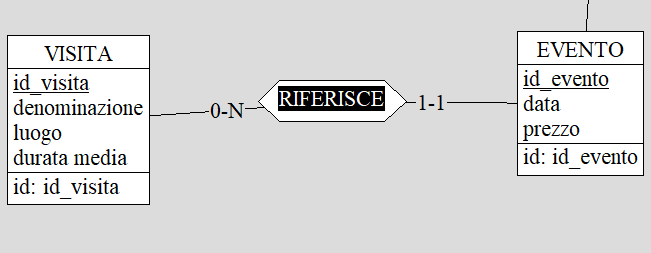
\includegraphics[width=0.99\textwidth]{visita-evento.png}
	\caption[short]{una visita può istanziare più eventi metre
		un evento riferisce per una determinata visita}
\end{figure}
\newpage
\chapter{Progettazione concettuale}
\section{Schema scheletro}
\section{Raffinamenti proposti}
\section{Schema concettuale finale}
\newpage
\chapter{Progettazione logica}
\section{Stima del volume dei dati}
\section{Descrizione delle operazioni principali e stima della loro frequenza}
\section{Schemi di navigazione e tabelle degli accessi}
\section{Raffinamento dello schema}
\section{Analisi delle ridondanze}
\section{Traduzione di entità e associazioni in relazioni}
\section{Schema relazionale finale}
\section{Traduzione delle operazioni in query SQL}
\newpage
\chapter{Progettazione dell'applicazione}
\end{document}
